\chapter[Resultados]{Resultados}

\section{Estrutura}
Com a utilização do programa CATIA V5 3D foi estruturado o sistema eletrônico acoplado a cadeira de rodas, \ref{fig:frontal}. Visando três preceitos básicos: comodidade, acessibilidade e conforto.

\begin{figure}[!htb]
\centering
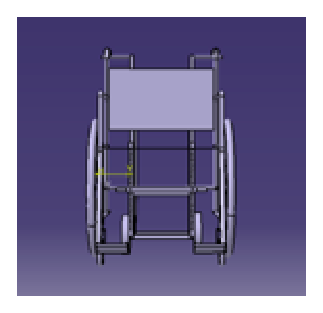
\includegraphics{figuras/estrutura/vista_frontal}
\caption{Vista Frontal}
\label{fig:frontal}
\end{figure}

O objetivo do projeto é desenvolver uma estrutura de fácil conexão e  resistente. O produto proposto, ver figura \ref{fig:traseira},\ref{fig:sistema}, \ref{fig:lateral} e \ref{fig:superior},deve se acoplar a qualquer cadeira de rodas. Foi pensado num dispositivo de um formato de uma mala para que seja de fácil conexão, uso e manuseio.

\begin{figure}[!htb]
\centering
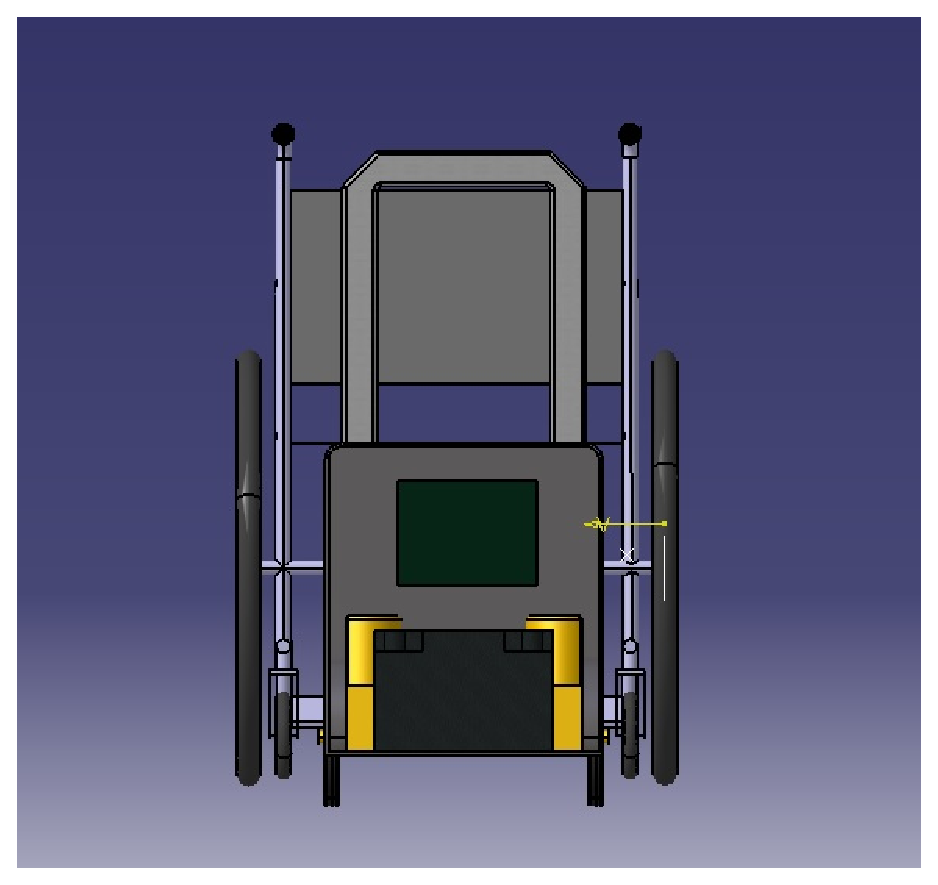
\includegraphics{figuras/estrutura/vista_traseira}
\caption{Vista Traseira}
\label{fig:traseira}
\end{figure}

\begin{figure}[!htb]
\centering
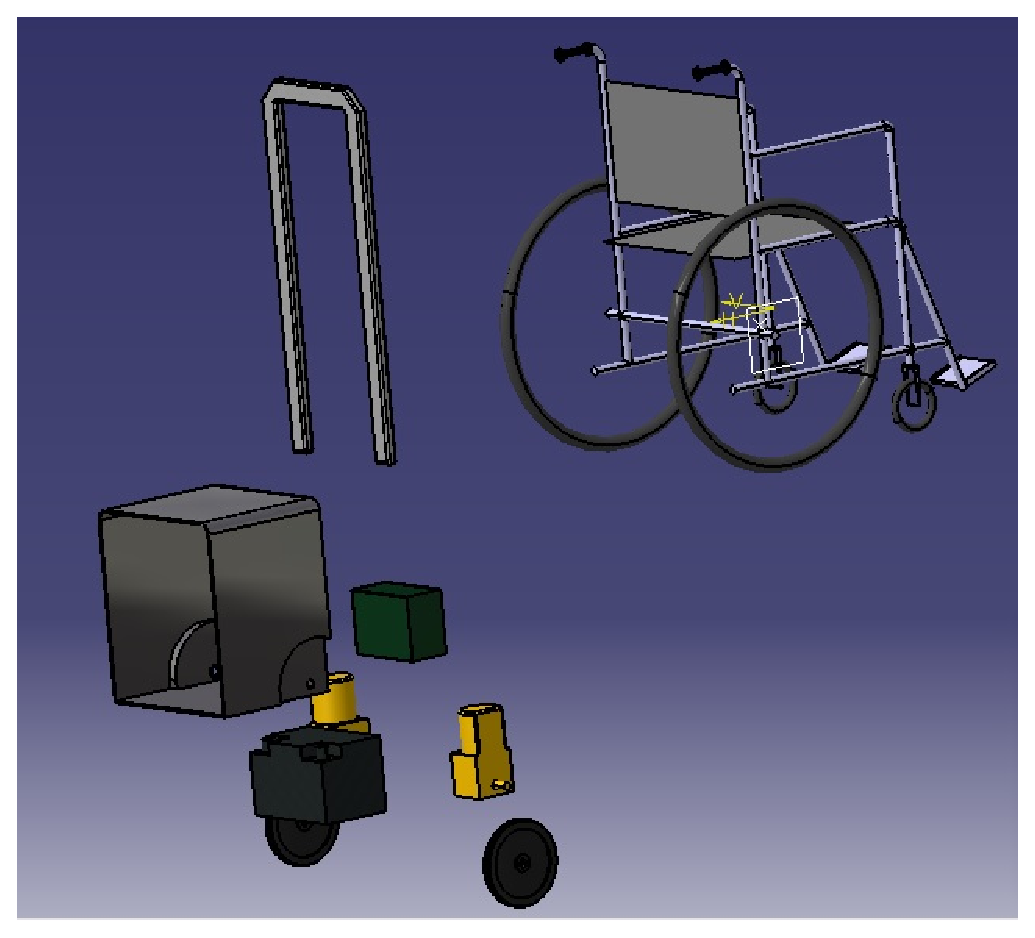
\includegraphics{figuras/estrutura/explode}
\caption{Visão do Sistema}
\label{fig:sistema}
\end{figure}

\begin{figure}[!htb]
\centering
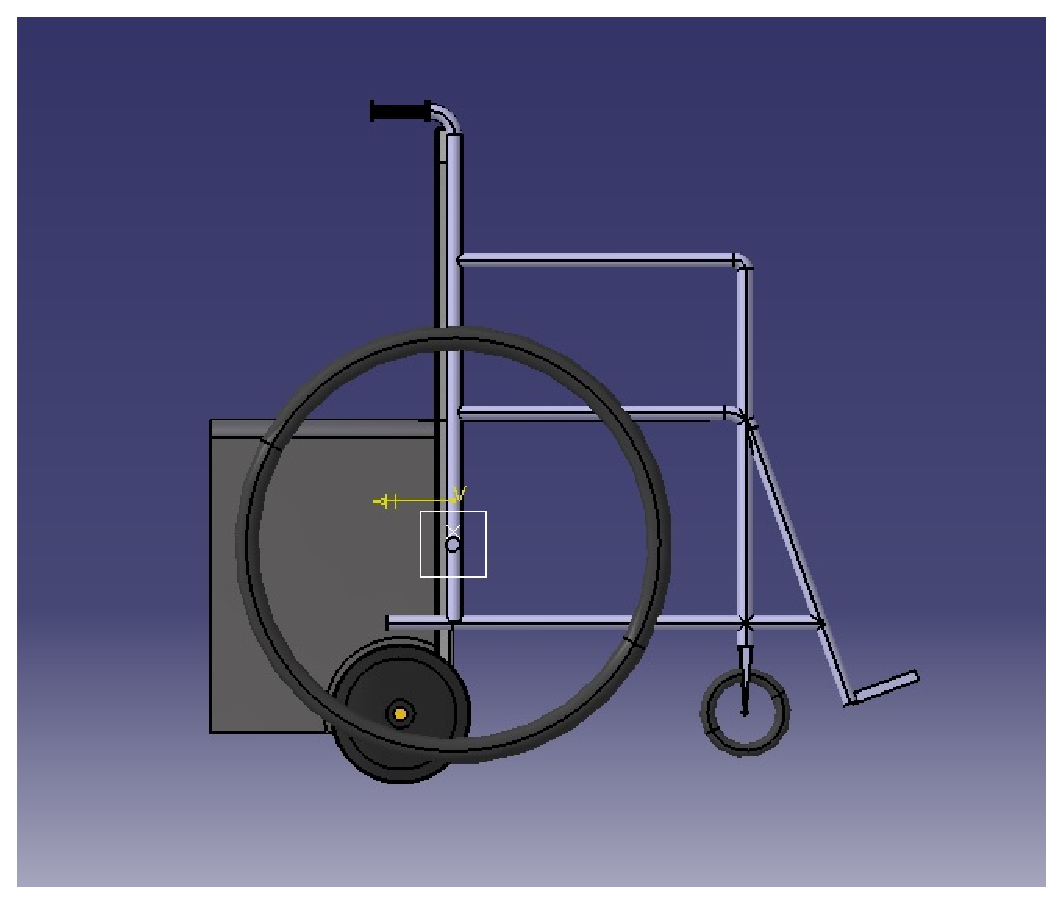
\includegraphics{figuras/estrutura/vista_lateral_cadeira}
\caption{Imagem Lateral}
\label{fig:lateral}
\end{figure}

\begin{figure}[!htb]
\centering
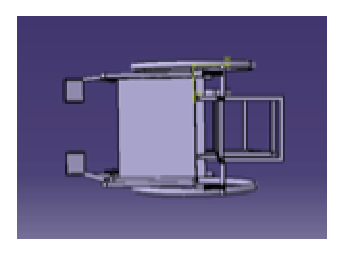
\includegraphics{figuras/estrutura/vista_superior}
\caption{Imagem Superior}
\label{fig:superior}
\end{figure}

\section{Power Train}

\subsection{Motor}
Será utilizado no projeto o motor de corrente continua. A escolha foi feita pois esse tipo de motor é muito utilizado em projetos que necessitam de velocidades variáveis, eles também apresentam uma região de torque e potência constante e são simples de realizar a aceleração e a desaceleração (HAMANAKA,2002). 

Especificações a serem atendidas:
\begin{itemize}
 \item Velocidade máxima de 7,2 km/h apx: 2m/s;
 \item Peso máximo de 120 kg;
 \item Peso da bateria 10 kg;
 \item Peso da cadeira (valor aproximado) 20kg;
 \item Peso total estimado: 150 Kg;
 \item Considerando hipoteticamente o coeficiente de atrito ($\mu$): 0,2.
\end{itemize}

\textbf{Força de atrito:}
\begin{equation}
 \overrightarrow{F} = \overrightarrow{N} * \mu = 150 * 9,8 * 0,2 = 294N
\end{equation}

\textbf{Potência do motor:}

\begin{equation}
 P_{x} = \frac{F * v}{100} = \frac{294 * 2}{1000} = \frac{588}{100} = 0,588kW
\end{equation}

O motor para a utilização na aplicação deve seguir algumas características dentro das especificações do projeto. Serão utilizados dois motores para motorizar a cadeira de rodas. Com isso é necessário que cada motor tenha a potência mínima de: \textbf{294W}.

\subsection{Baterias}
\subsubsection{Chumbo-Ácido}
Inventadas em 1859 pelo físico francês Gaston Planté, é muito utilizada hoje em dia em diferentes áreas, como automóveis, sistemas de fornecimento de energia elétrica ininterrupta (no-breaks) e cadeiras de rodas elétricas. Desprezando o problema do peso, é a bateria mais econômica.

Um grande problema foi solucionado na década de 70, onde pesquisadores conseguiram desenvolver uma bateria de chumbo-ácido livre de manutenção, podendo operar em qualquer posição. Nesta bateria, o invólucro foi selado e o eletrólito líquido foi transformado em separadores umedecidos.

As baterias SLA (bateria selada chumbo-ácido), também conhecida como Gelcell, tem uma faixa típica de capacidade que vai de 0,2 Ah até 30 Ah. Esse tipo de bateria está livre do famoso efeito memória, e deixar a bateria em carga flutuante por um longo período não causa nenhum dano.

A bateria de chumbo-ácido tem a melhor retenção de carga entre todas as baterias recarregáveis. As baterias de SLA descarregam aproximadamente 40\% da sua energia armazenada em média em 1 ano, já uma de NiCd se auto descarrega na mesma quantidade em 3 meses.

As baterias SLA devem sempre ser armazenadas carregadas. Deixar a bateria descarregada causa sulfação, uma condição que torna difícil, se não impossível, de se recarregar as baterias. A bateria SLA consegue fornecer entre 200 e 300 ciclos de carga/descarga.

Vantagens:
\begin{itemize}
 \item A mais barata em termos de custo por watt horas;
 \item Segura e durável quando utilizada corretamente;
 \item Auto descarga está entre as mais baixas entre as baterias com sistema de recarga;
 \item Não exige muita manutenção e não tem o efeito memória.
\end{itemize}

Limitações:
\begin{itemize}
 \item A bateria não pode ser armazenada em completa descarga, a tensão tem de estar acima de 2,10V;
 \item Densidade baixa da energia;
 \item Ciclo de carga/descarga limitado;
 \item O eletrólito e o conteúdo da carga podem causar danos ambientais;
 \item Imprópria para dispositivos de mão que exigem tamanho compacto. 
\end{itemize}

\subsubsection{Carregando Baterias Chumbo-Ácido}
O tempo de carga de uma bateria de Chumbo-Ácido (selada) é de 12 a 16 horas. Com correntes de carga maiores, e métodos de carga multi-estágios, o tempo de carga pode ser reduzido para 10 horas ou menos.

Durante a carga em corrente constante, a bateria carrega 70\% em aproximadamente 5 horas; os 30\% restantes são completados por uma lenta carga de pico. A corrente de pico dura outras 5 horas e é essencial para o bem estar da bateria. 

A bateria escolhida para o projeto foi uma bateria de chumbo ácido, muito utilizado em veículos devido seu fácil acesso e baixo custo. Atualmente ela já é utilizada em cadeiras de rodas elétricas. Este é o tipo menos eficiente de bateria, com a pior relação peso/energia, mas em compensação é a tecnologia mais barata.

\textbf{Autonomia}
A capacidade de armazenamento de energia de uma bateria é medida através da multiplicação da corrente de descarga pelo tempo de autonomia, sendo dado em Ampére-hora (Ah).

Cálculo da autonomia da bateria em horas:

$Autonomia(h) = \frac{Capacidade da bateria(Ah)}{Consumo do circuito(A)}$

Potencia é dada por: 
\begin{equation}
 P=U*I
\end{equation}

Para o projeto é necessário 2 motores de no mínimo 294W, ou seja, os motores puxaram uma potência de 588W e são motores de 12V, com isso a corrente necessária é de: 588 = 12 * I \rightarrow I = $\frac{588}{12}$ = 49A

O modelo e as características da bateria foram informadas abaixo:

\begin{itemize}
 \item Bateria GetPower;
 \item Bateria de gel selada;
 \item Tensão: 12V;
 \item Capacidade: 26Ah;
 \item Peso: 8,6 Kg;
 \item Dimensões ( Comp x Larg x Alt ) : 166 x 175 x 125mm;
 \item Preço: R\$240,00(Mercado livre).
\end{itemize}

\subsection{Interface com o usuário}

Desde a primeira patente de cadeira de rodas elétrica em 1940 [1], diversos modelos de cadeiras de rodas motorizadas foram desenvolvidos. As mais diversas interfaces humano-computador foram criadas de modo a facilitar a vida do cadeirante, desde cadeiras elétricas com um joystick simples à cadeiras inteligentes controladas por voz ou sem fio via celular, com monitoramento de velocidade, bateria e inclinação [4]. Foram pesquisas várias formas de controle de cadeiras de rodas que podem ser consultados na tabela 1.

COLOCAR IMAGEM TABELA 1

\subsection{Dispositivo de controle}
Um mapeamento feito pelos integrantes da equipe sobre como a Cadeira de Rodas automatizada será feita pode ser observada na figura 1.

Nesse esquemático pode ser observado que a interface com o usuário recebe um input do usuário, utilizando Joystick ou Aplicativo. O sinal emitido por esta interface será processado em um \textit{raspeberry pi}, que por consequência irá movimentar o motor.

COLOCAR IMAGEM RASP

\subsubsection{Joystick}
Um joystick é um periférico de computador pessoal ou um dispositivo geral de controle que consistem em uma vara vertical na qual os pivôs se aproximam de uma extremidade e transmitem seu ângulo em duas ou três dimensões a um computador[3]. O Joystick, muito utilizado em computadores e jogos eletrônicos provou sua utilidade em diversas áreas. 

Para as cadeiras de rodas automatizadas essa é uma solução comum de controle para as mesmas, tendo em vista que é relativamente simples de ser acoplado uma vez que se entenda seu funcionamento básico.

Para o projeto em questão essa foi uma das alternativas encontradas. No qual o joystick seria acoplado ao braço da cadeira, ou em uma posição que o usuário se sinta mais ergonomicamente confortável. Este acoplamento deve ser simples para favorecer a característica de portabilidade do projeto como um todo.

Caso necessário a conexão do joystick ao sistema de controle pode ser feita por bluetooth, tal característica contribui para o objetivo final do projeto.[6]

\subsubsection{Smartphone}
Um telefone smartphone é um telefone celular com um sistema operacional móvel avançada que combina as características de um sistema operacional de computador pessoal com outros recursos úteis para uso móvel ou portátil [8].

Devido á portabilidade destes dispositivos e sua facilidade de integração com outros sistemas, uma possível solução para a interação do usuário com o sistema pode ser feita. Uma conexão entre o dispositivo e o sistema será feita através de Bluetooth (Android ) ou "Virtual Private Network" (iOS e Android). 

Para o projeto em questão o usuário pode optar por utilizar o "Smartphone" ou ainda utilizar o joystick.

\subsubsection{Protótipo}

COLOCAR IMAGEM PROTÓTIPOS

O protótipo na figura(prototipos) foi feito com o intuito de mostrar o fluxo do aplicativo sugerido para o controle da cadeira de rodas automatizada. 

\subsection{Tecnologias}

\subsubsection{Raspeberry Pi}

É um componente eletrônico que será responsável pelo controle do motor, seu modelo ainda será decidido. A escolha foi feita devido ao número de recursos oferecidos e o baixo custo desse componente. 

O Raspberry  tem como principal componente um pequeno circuito integrado que reúne o processador com a arquitetura ARM, a GPU VideoCore IV e a memória RAM que é compativel com o sistema operacional GNU/Linux. Suas especificações gerais são:

\begin{itemize}
 \item Processador ARM 11 de 700 MHz;
 \item GPU VideoCore IV de 250 MHz;
 \item 256 MB total de RAM;
 \item Saída de Vídeo HDMI e RCA;
 \item Saída de áudio P2;
 \item Interface de rede ethernet;
 \item 2 portas USB;
 \item Conector Micro USB para alimentação (5 volts, 700mA).
\end{itemize}

A figura(referencia ao rasp) corresponde ao esquemático dos componentes do raspeberry que será utilizado no projeto.

COLOCAR IMAGEM DA RASP

\subsubsection{Linguagem de programação}

Uma das linguagens a ser adotada será Python devido a facilidade de existir bibliotecas específicas que controlam o GPIO (General Purpose Input/Output) do Raspberry Pi.

Essa linguagem é uma linguagem de programação de alto nivel, interpretada, orientada a objetos, de tipagem dinamica. Tem uma sintax consisa e clara, juntamente com uma biblioteca com recursos poderosos. Os módulos e frameworks ainda não foram decididos.



 










